
\documentclass[10pt, sans, compress, usenames, dvipsnames, aspectratio=169]{beamer}

%% Import the template configuration
\usepackage[T1]{fontenc}
\usepackage{lmodern}
\usepackage{graphicx}
\usepackage[french]{babel}
\usepackage[utf8]{inputenc}
\usetheme{Warsaw}
\usepackage{wasysym}
\usepackage{tabularx}
\usepackage{hyperref}
\usepackage[absolute,overlay]{textpos}
\setbeamertemplate{navigation symbols}{}
\useoutertheme{infolines}
\useinnertheme{rectangles}
\setbeamertemplate{background canvas}{
\includegraphics[width=\paperwidth,height=\paperheight]{images/ucabackground-16_9.png}}
\usepackage{caption}
\captionsetup{figurename=}
\definecolor{uca01}{HTML}{006E83}
\definecolor{uca02}{HTML}{0096A0}
\definecolor{uca03}{HTML}{006C82}
\definecolor{uca04}{HTML}{0398A1}
\definecolor{uca05}{HTML}{585656}
\definecolor{uca06}{HTML}{438D97}
\definecolor{grisuca}{HTML}{5E5C5C}


\setbeamercolor{palette primary}{bg=uca06}
\setbeamercolor{palette secondary}{bg=uca03}
\setbeamercolor{palette tertiary}{bg=uca04}
\setbeamercolor{palette quaternary}{bg=uca05}
\setbeamercolor{block title}{bg=uca06}
\setbeamercolor{itemize item}{fg=uca03}
\setbeamercolor{itemize subitem}{fg=uca03}
\setbeamercolor{itemize subsubitem}{fg=uca03}


\setbeamercolor{enumerate item}{bg=uca03,fg=uca03}
\setbeamercolor{enumerate subitem}{bg=uca03,fg=uca03}
\setbeamercolor{enumerate subsubitem}{bg=uca03,fg=uca03}
\setbeamercolor{enumerate mini template}{bg=uca03,fg=uca03}
\setbeamercolor{itemize body}{fg=uca03}
\setbeamercolor{itemize subbody}{fg=uca03}
\setbeamercolor{itemize subsubbody}{fg=uca03}
\setbeamercolor{enumerate body}{fg=uca03}
\setbeamercolor{enumerate subbody}{fg=uca03}
\setbeamercolor{enumerate subsubbody}{fg=uca03}

\setbeamercolor{item projected}{bg=uca03}
\setbeamercolor{section in toc}{fg=grisuca}
\setbeamercolor{normal text}{fg=grisuca}



\title{FAIR Bioinfo 2022}
\subtitle{Best practice in your bioinformatic projects\blfootnote{This work is based on the IFB and I2BC formation offer}}
\author[Pierre MARIN]{\underline{P. Marin}, M. Hiriart, P. Ruiz \& N. Goué\\\texttt{aubi@uca.fr}}
\institute{Université Clermont Auvergne, AuBi, Mésocentre}
\date{\today}
\newif\iflattersubsect

\begin{document}

\begin{frame}
  \titlepage
  \begin{textblock*}{5cm}(2cm,0.5cm) % {block width} (coords)
  
\includegraphics[width=2.3cm,height=1.3cm]{images/logo_ifb.pdf}
  \end{textblock*}
  \begin{textblock*}{5cm}(13cm,0.3cm) % {block width} (coords)
  
\includegraphics[width=1.5cm,height=1.5cm]{images/i2bc.png}
  \end{textblock*}
  \begin{textblock*}{5cm}(1cm,4cm) % {block width} (coords)
  
\includegraphics[width=3.5cm,height=3cm]{images/logoAuBi-2019.pdf}
  \end{textblock*}
  \begin{textblock*}{5cm}(12cm,3.6cm) % {block width} (coords)
  
\includegraphics[width=3.5cm,height=3cm]{images/mesocentre.png}
  \end{textblock*}
   \begin{textblock*}{5cm}(12.8cm,6cm) % {block width} (coords)
  
\includegraphics[width=2cm,height=1cm]{images/medis_logo.png}
  \end{textblock*}
\end{frame}
%\begin{frame}
%  \frametitle{Sommaire}
%   \tableofcontents
%\end{frame}


\section{A reproducibility crisis}
%% THE CRISIS PART %%
\begin{frame}
\centering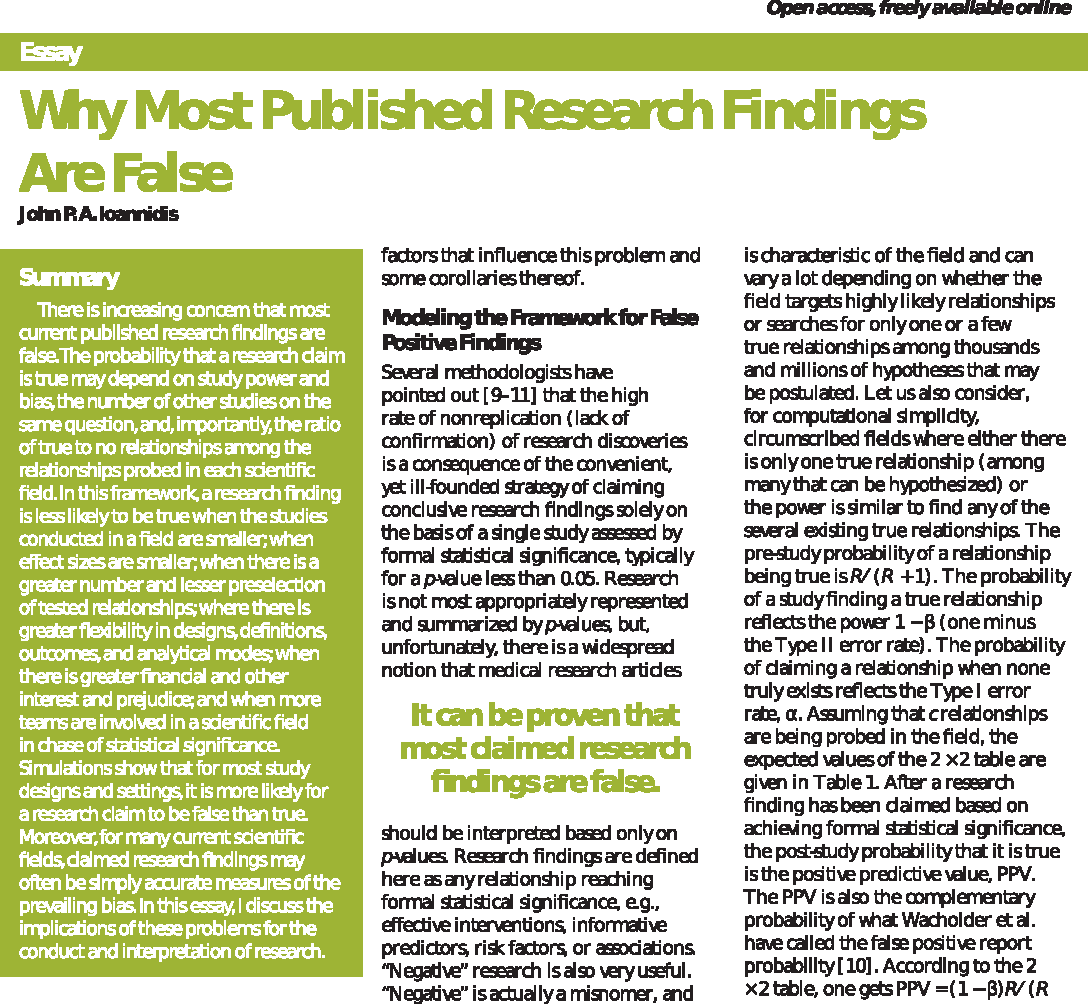
\includegraphics[scale=0.5]{reproduce_crisis_paper.pdf}
\blfootnote{\url{https://doi.org/10.1371/journal.pmed.0020124}}
\end{frame}

\begin{frame}
\begin{block}{Crisis elements}
\begin{itemize}
\item Highlighted around 2005
\item Since 2010 more articles related to the non reproducibility
\item Medecine is one of the most impacted discipline
\end{itemize}
\end{block}
\end{frame}

%% SLIDE CRISIS FROM IFB %%

\begin{frame}
\includegraphics[page=4,scale=0.55]{01_OS_and_FAIR_intro.pdf}
\blfootnote{\url{https://doi.org/10.1038/533452a}}
\end{frame}

\begin{frame}
\includegraphics[page=5,scale=0.55]{01_OS_and_FAIR_intro.pdf}
\blfootnote{\url{http://reproducibility.cs.arizona.edu/v2/data/Total.png}}
\end{frame}

\begin{frame}
\includegraphics[page=6,scale=0.5]{01_OS_and_FAIR_intro.pdf}
\blfootnote{\url{https://retractionwatch.com/the-retraction-watch-leaderboard}}
\end{frame}

\begin{frame}
\includegraphics[page=7,scale=0.55]{01_OS_and_FAIR_intro.pdf}
\end{frame}


\section{Open science and FAIR}
%%%% FAIR history

\begin{frame}
\begin{block}{FAIR history}
\begin{itemize}
\item Born in 2016 with \textit{The FAIR Guiding Principles for scientific data management and stewardship}
\item How to build, stock, share, use and publish data
\item Make criteria to better use our data
\end{itemize}
\end{block}
\blfootnote{\url{https://doi.org/10.1038/sdata.2016.18}}
\end{frame}

\begin{frame}
\centering{
\includegraphics[scale=0.5]{fair_paper_2016_crop.pdf}}
\blfootnote{\url{https://doi.org/10.1038/sdata.2016.18}}
\end{frame}

% FAIR for data and tools
\begin{frame}
\begin{block}{Apply FAIR TO}
\begin{itemize}
\item Your DATA
	\begin{itemize}
	\item Data lifecycle
	\item Data Management Plan (DMP)
	\item Metadata
	\item Data storage
	\end{itemize}
\end{itemize}
\end{block}
\end{frame}

% la perte des données dans le temps
\begin{frame}{Focus on the data lifecycle}
\only<1>{\centering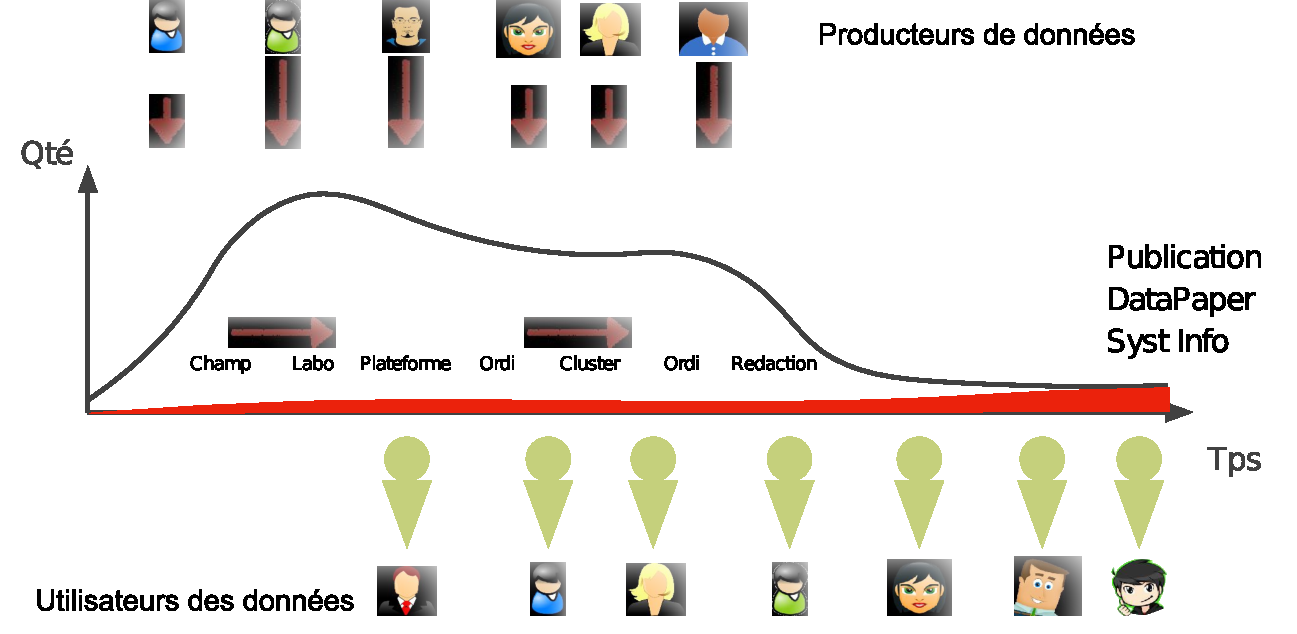
\includegraphics[scale=0.55]{fair_data_introduction_datalife.pdf}}
\only<2>{\centering\includegraphics[page=4,scale=0.4]{03_Organiser_son_projet_Juin_2022.pdf}}

\end{frame}

\begin{frame}{Focus on the data lifecycle}
\centering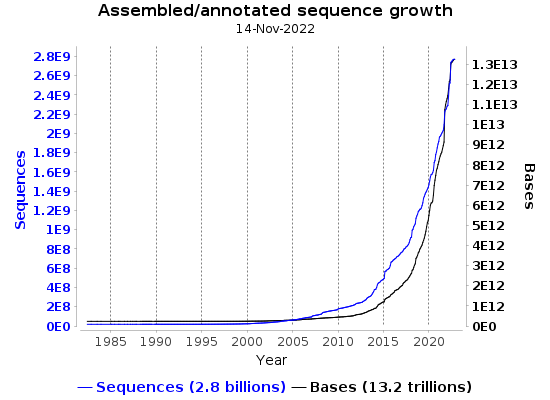
\includegraphics[scale=0.50]{ena_embl_growth.png}
\blfootnote{\url{https://www.ebi.ac.uk/ena/browser/about/statistics}}
\end{frame}

\begin{frame}{Focus on the data exchange}
\centering\includegraphics[page=14,scale=0.45]{03_Organiser_son_projet_Juin_2022.pdf}
\end{frame}

\begin{frame}
\centering
\includegraphics[page=1,scale=0.4]{Cost-Benefit-analysis-for-FAIR.pdf}
\end{frame}

\begin{frame}
\begin{block}{Apply FAIR TO}
\begin{itemize}
\item Your DATA
	\begin{itemize}
	\item Data lifecycle
	\item Data Management Plan (DMP)
	\item Metadata
	\item Data storage
	\end{itemize}
\item Your scripts, environment...
	\begin{itemize}
	\item Objective of this training
	\end{itemize}
\end{itemize}
\end{block}
\end{frame}


%%%% Findable
\begin{frame}
\centering\includegraphics[page=8,scale=0.55]{01_OS_and_FAIR_intro.pdf}
\end{frame}


\begin{frame}
\centering
\includegraphics[scale=0.5]{404_error.png}
\end{frame}


\begin{frame}
\begin{block}{To be Findable}
\begin{itemize}
\item (meta)data are assigned a globally unique and persistent identifier
\item data are described with rich metadata
\item metadata clearly and explicitly include the identifier of the data it describes
\item (meta)data are registered or indexed in a searchable ressource
\end{itemize}
\end{block}
\end{frame}

%%%% ACCESSIBLE
\begin{frame}
\includegraphics[page=9,scale=0.55]{01_OS_and_FAIR_intro.pdf}
\end{frame}

\begin{frame}
\begin{block}{To be Accessible}
\begin{itemize}
\item (meta)data are retrievable by their identifier using a standardized communication protocol
\item the protocol is open, free, and universally implementable
\item the protocol allows for an authentication and authorization procedure, where necessary
\item metadata are accessible, even when the data are no longer available
\end{itemize}
\end{block}
\end{frame}

%%%% INTEROPERABLE
\begin{frame}
\includegraphics[page=10,scale=0.55]{01_OS_and_FAIR_intro.pdf}
\end{frame}

\begin{frame}
\begin{block}{To be Interoperable}
\begin{itemize}
\item (meta)data use a formal, accessible, shared, and broadly applicable language for knowledge representation.
\item (meta)data use vocabularies that follow FAIR principles
\item (meta)data include qualified references to other (meta)data
\end{itemize}
\end{block}
\end{frame}

%%%% REUSABLE
\begin{frame}
\includegraphics[page=11,scale=0.55]{01_OS_and_FAIR_intro.pdf}
\end{frame}

\begin{frame}
\begin{block}{To be Reusable}
\begin{itemize}
\item meta(data) are richly described with a plurality of accurate and relevant attributes
\item (meta)data are released with a clear and accessible data usage license
\item (meta)data are associated with detailed provenance
\item (meta)data meet domain-relevant community standard
\end{itemize}
\end{block}
\end{frame}

\begin{frame}
\centering\includegraphics[page=12,scale=0.6]{01_OS_and_FAIR_intro.pdf}
\end{frame}


\begin{frame}{A complete integrated FAIR environment}{The Galaxy project}
\centering
\includegraphics{galaxylogo.pdf}
\end{frame}

\begin{frame}{A complete integrated FAIR environment}{The Galaxy project}
\begin{block}{Galaxy}
Galaxy is an open-source platform for FAIR data analysis that enables users to:
\begin{itemize}
\item Use tools from various domains (that can be plugged into workflows) through its graphical web interface.
\item Run code in interactive environments (RStudio, Jupyter...) along with other tools or workflows.
\item Manage data by sharing and publishing results, workflows, and visualizations.
\item Ensure reproducibility by capturing the necessary information to repeat and understand data analyses.
\end{itemize}
\end{block}
\end{frame}


\begin{frame}{A complete integrated FAIR environment}{The Galaxy project}
\only<1>{\centering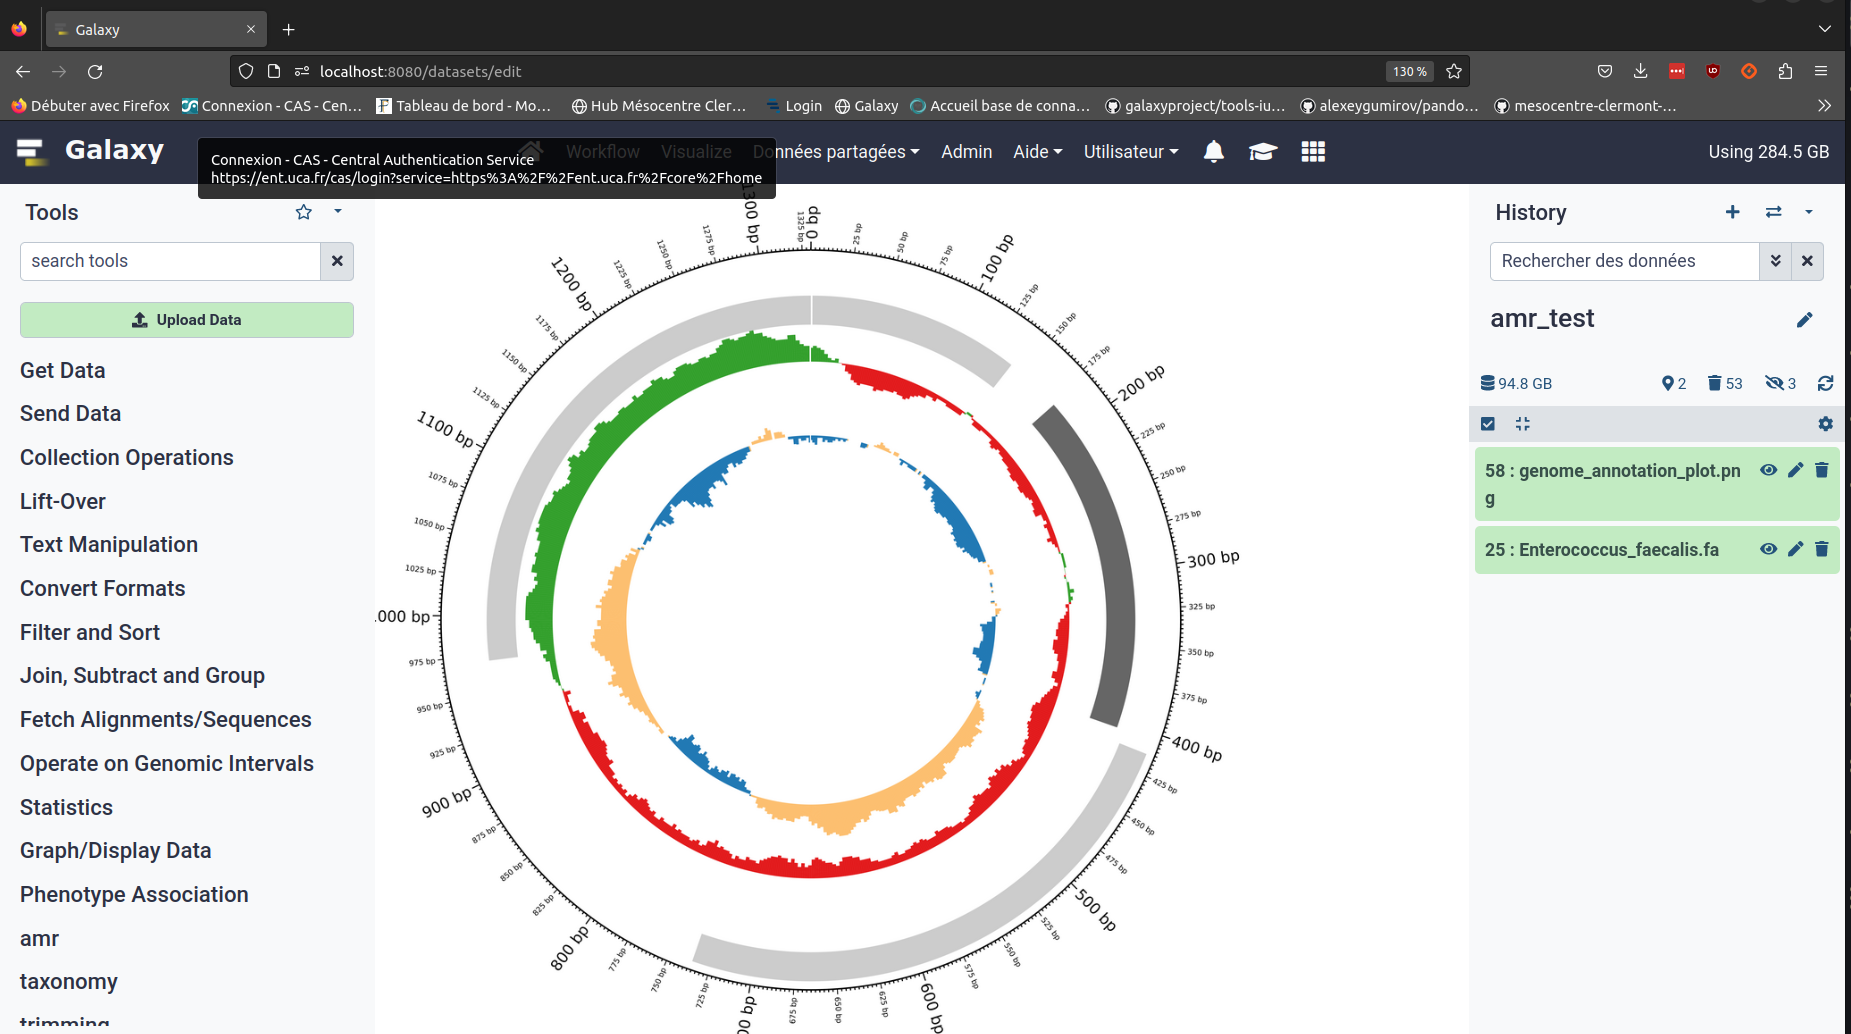
\includegraphics[scale=0.2]{galaxy_screen1.png}}
\only<2>{\centering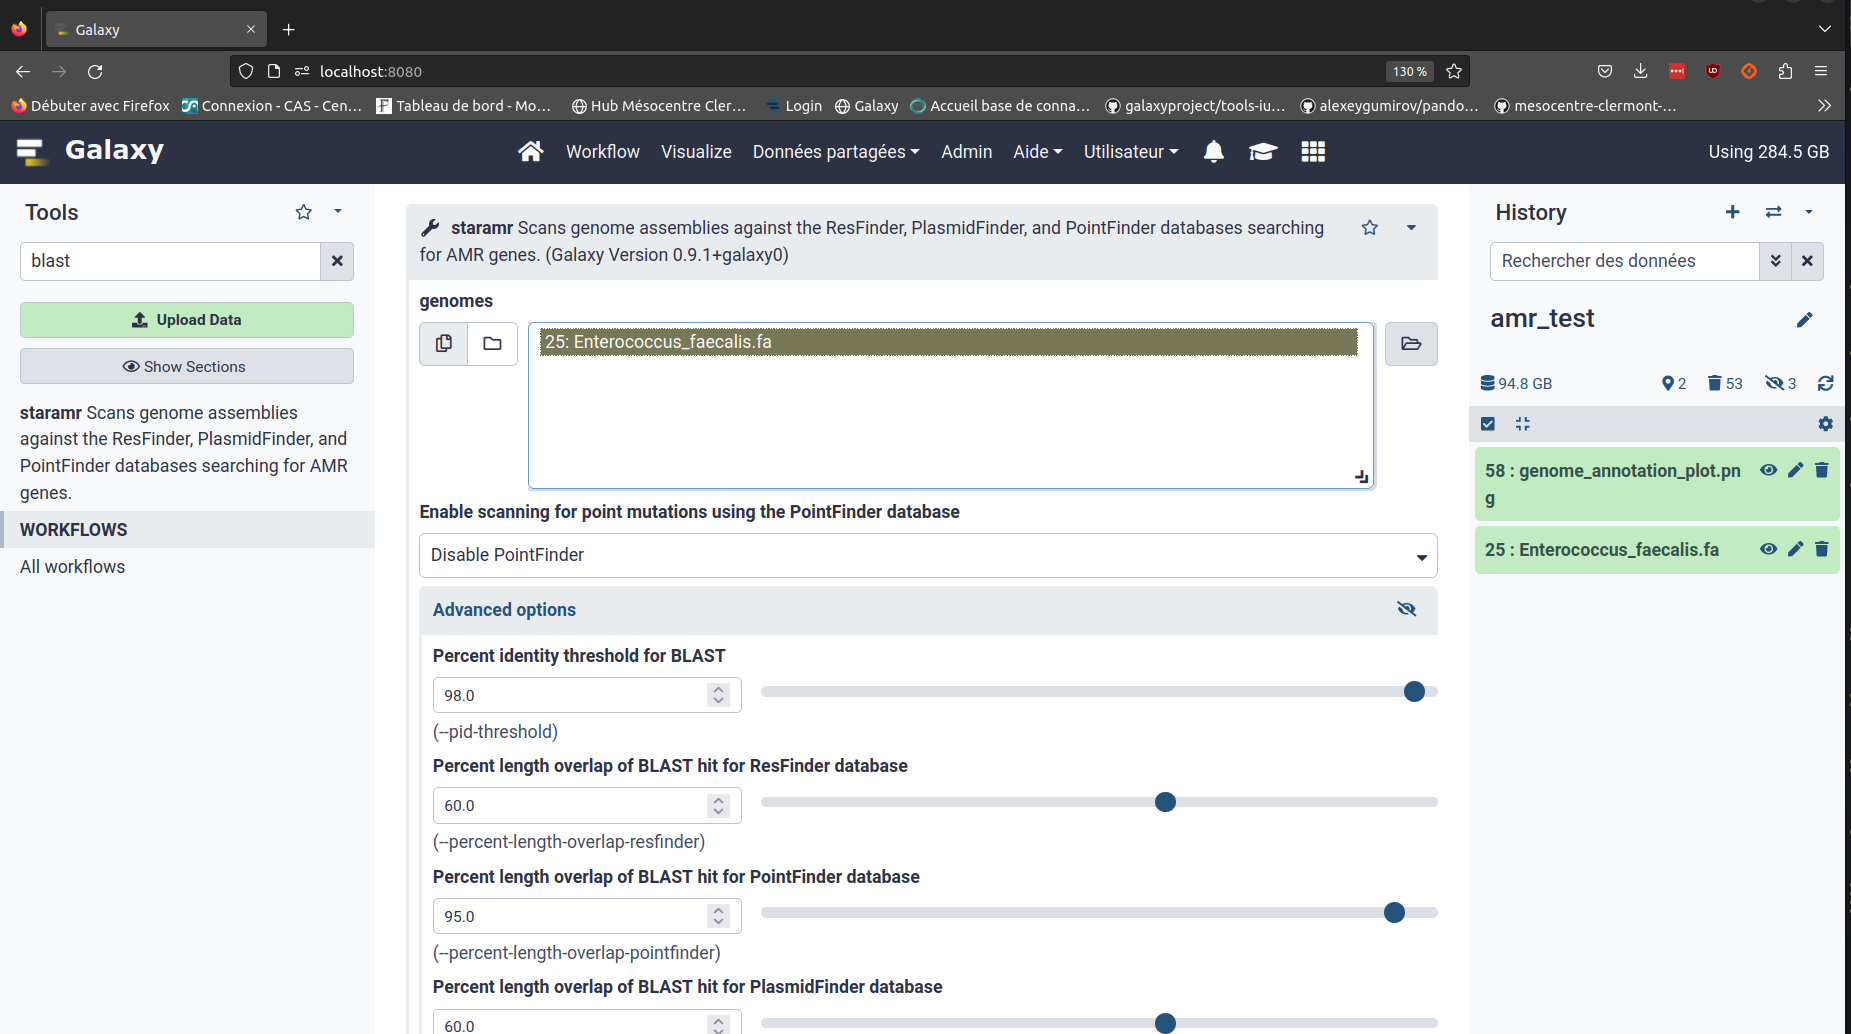
\includegraphics[scale=0.2]{galaxy_screen2.png}}
\only<3>{\centering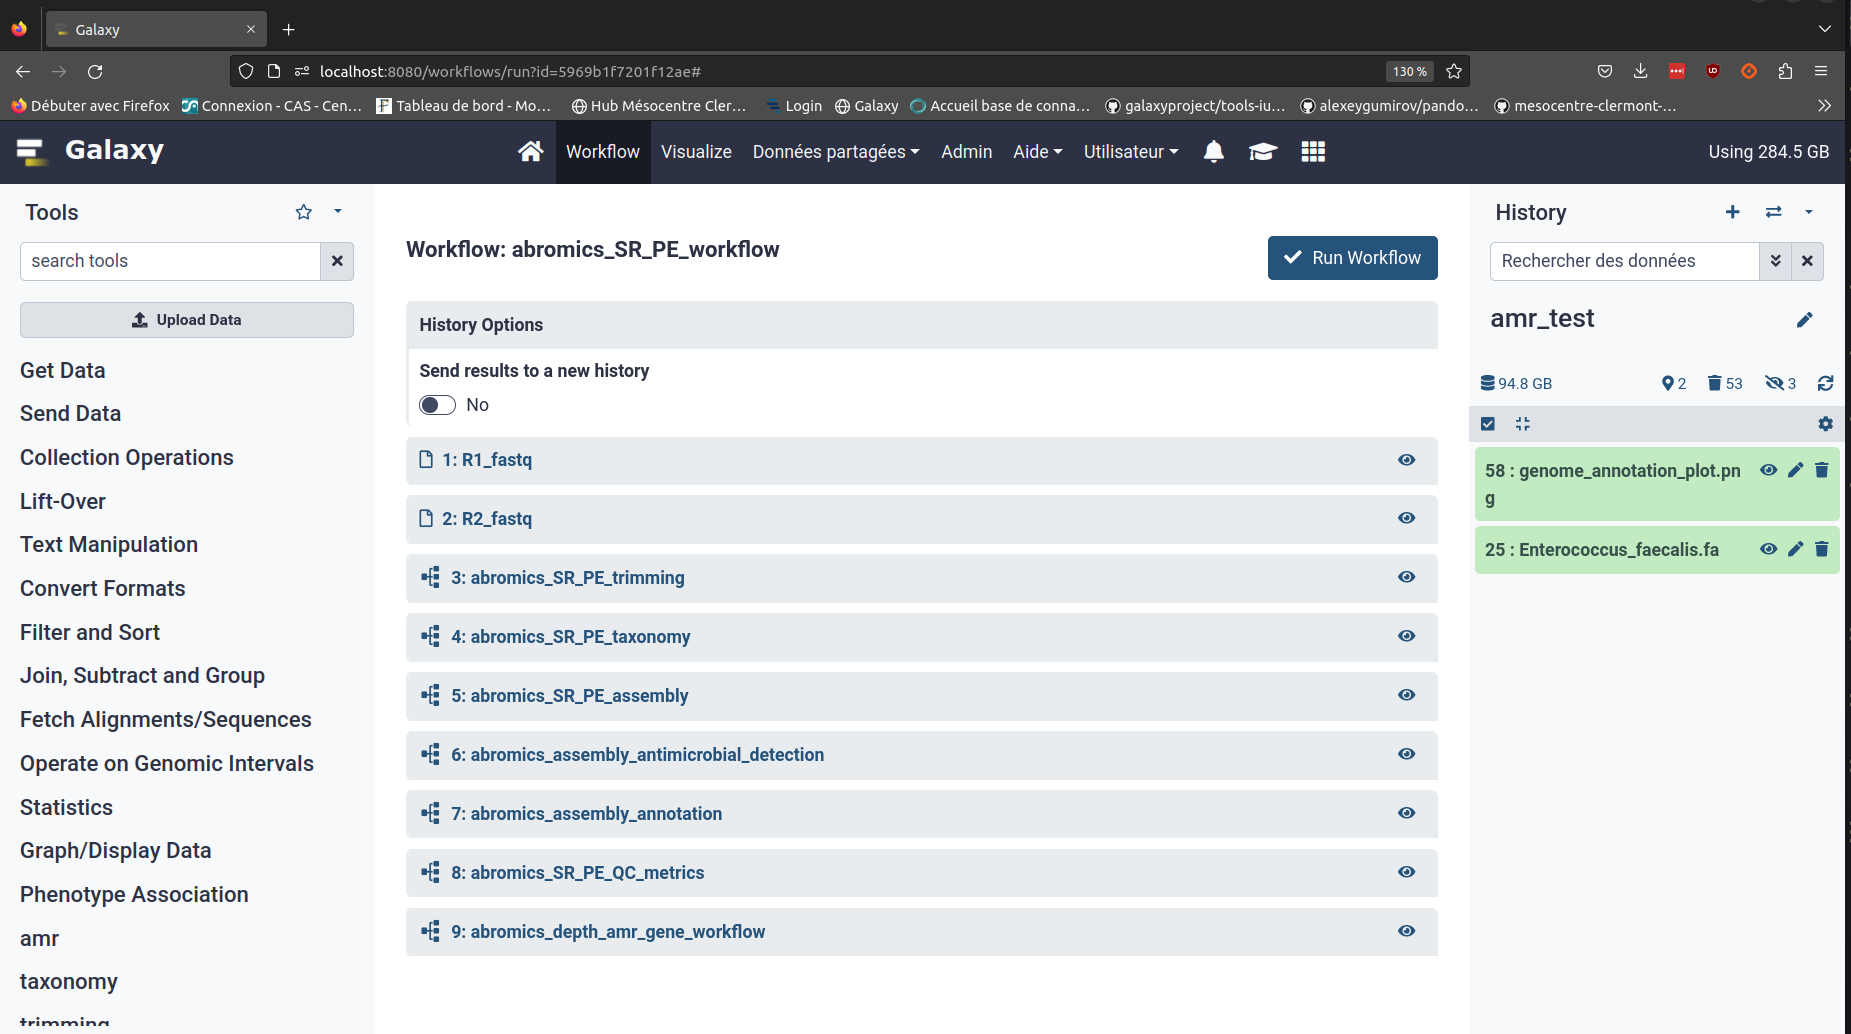
\includegraphics[scale=0.2]{galaxy_screen3.png}}
\only<4>{\centering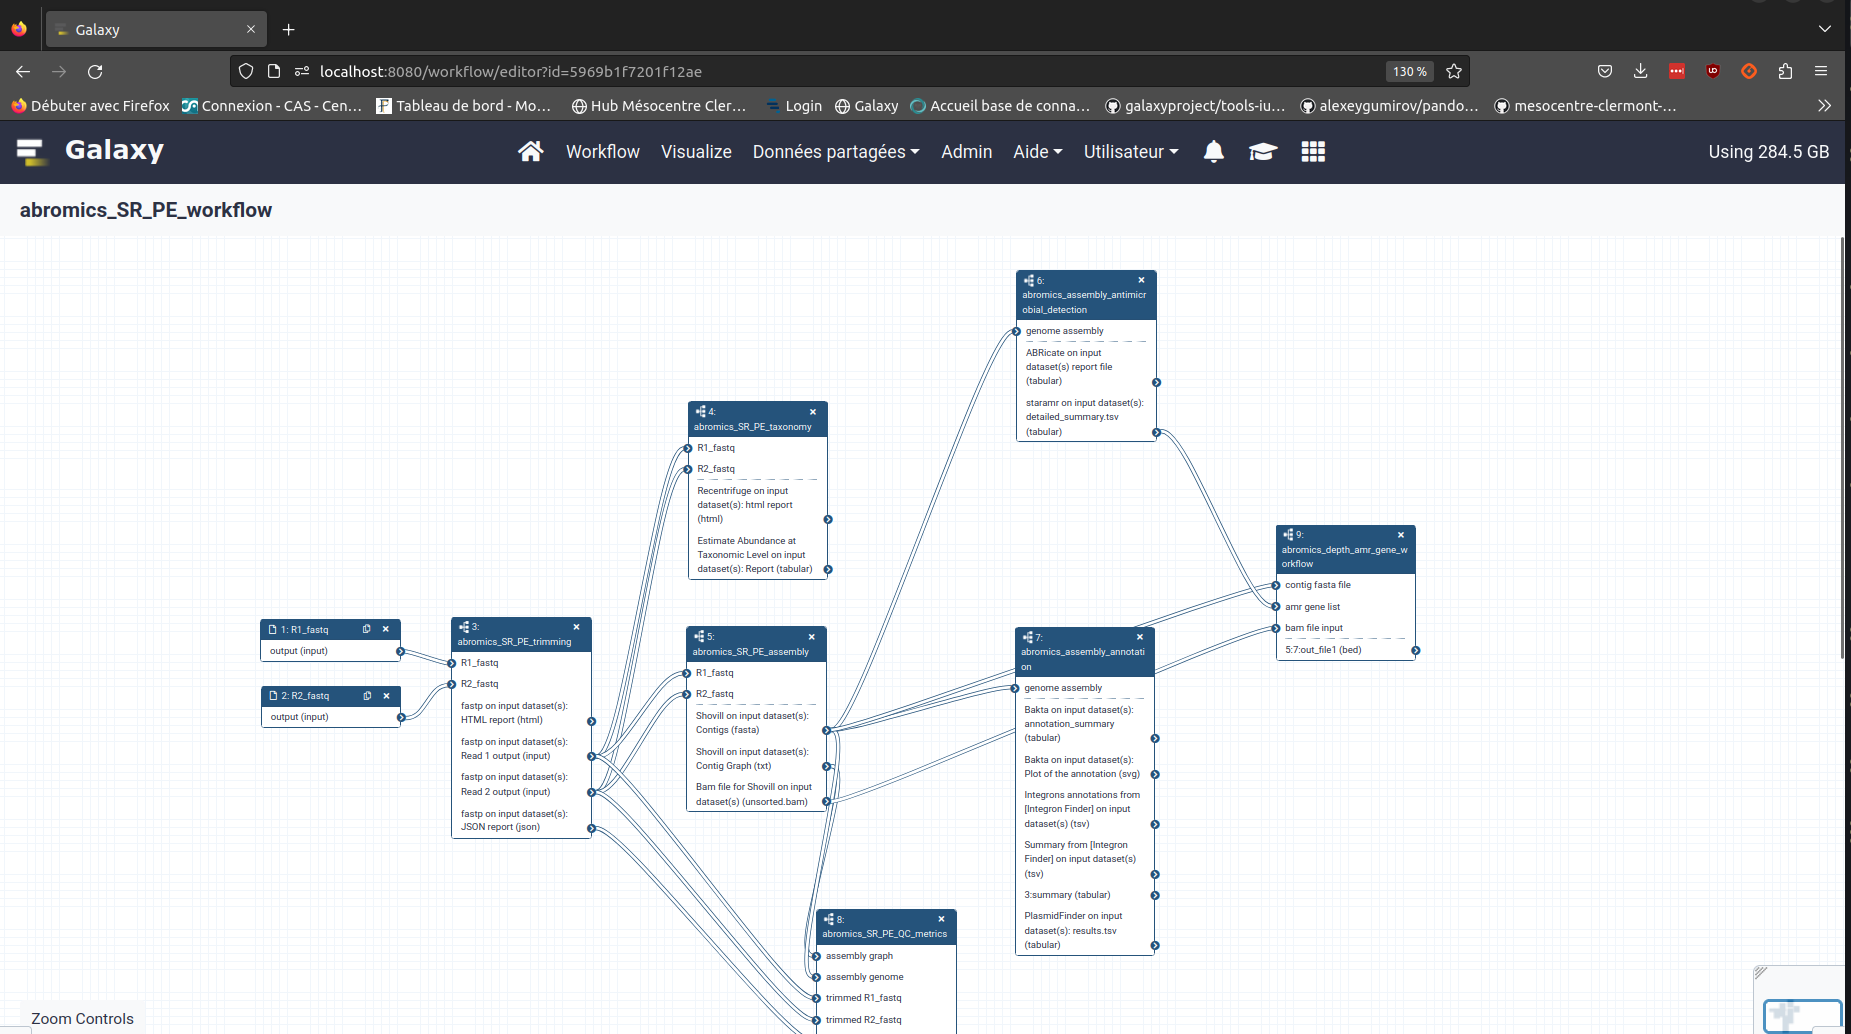
\includegraphics[scale=0.2]{galaxy_screen4.png}}
\end{frame}

\begin{frame}{A FAIR approach at any level}
\onslide<1->{
\centering
\includegraphics[scale=0.08]{One_Ring_inscription.pdf}
\newline
\textit{"One practice to rule them all, One practice to find them, One practice to bring them all and in the FAIR bind them."}
}
\onslide<2->{
\begin{block}{Improvement for who?}
At each level a good practice help you
\begin{itemize}
	\item Long term efficiency to a bioinformatician
	\item stop wasting time for a beginner
\end{itemize}
\end{block}
}
\end{frame}

\begin{frame}{How to integrate FAIR concepts in my work ?}{Some tools for reproducible research}
\begin{itemize}
\item {\sout{\color{gray} FAIR apply on the data}}
\item FAIR apply into the code
\end{itemize}
\begin{textblock*}{15cm}(5cm,1.5cm) % {block width} (coords)
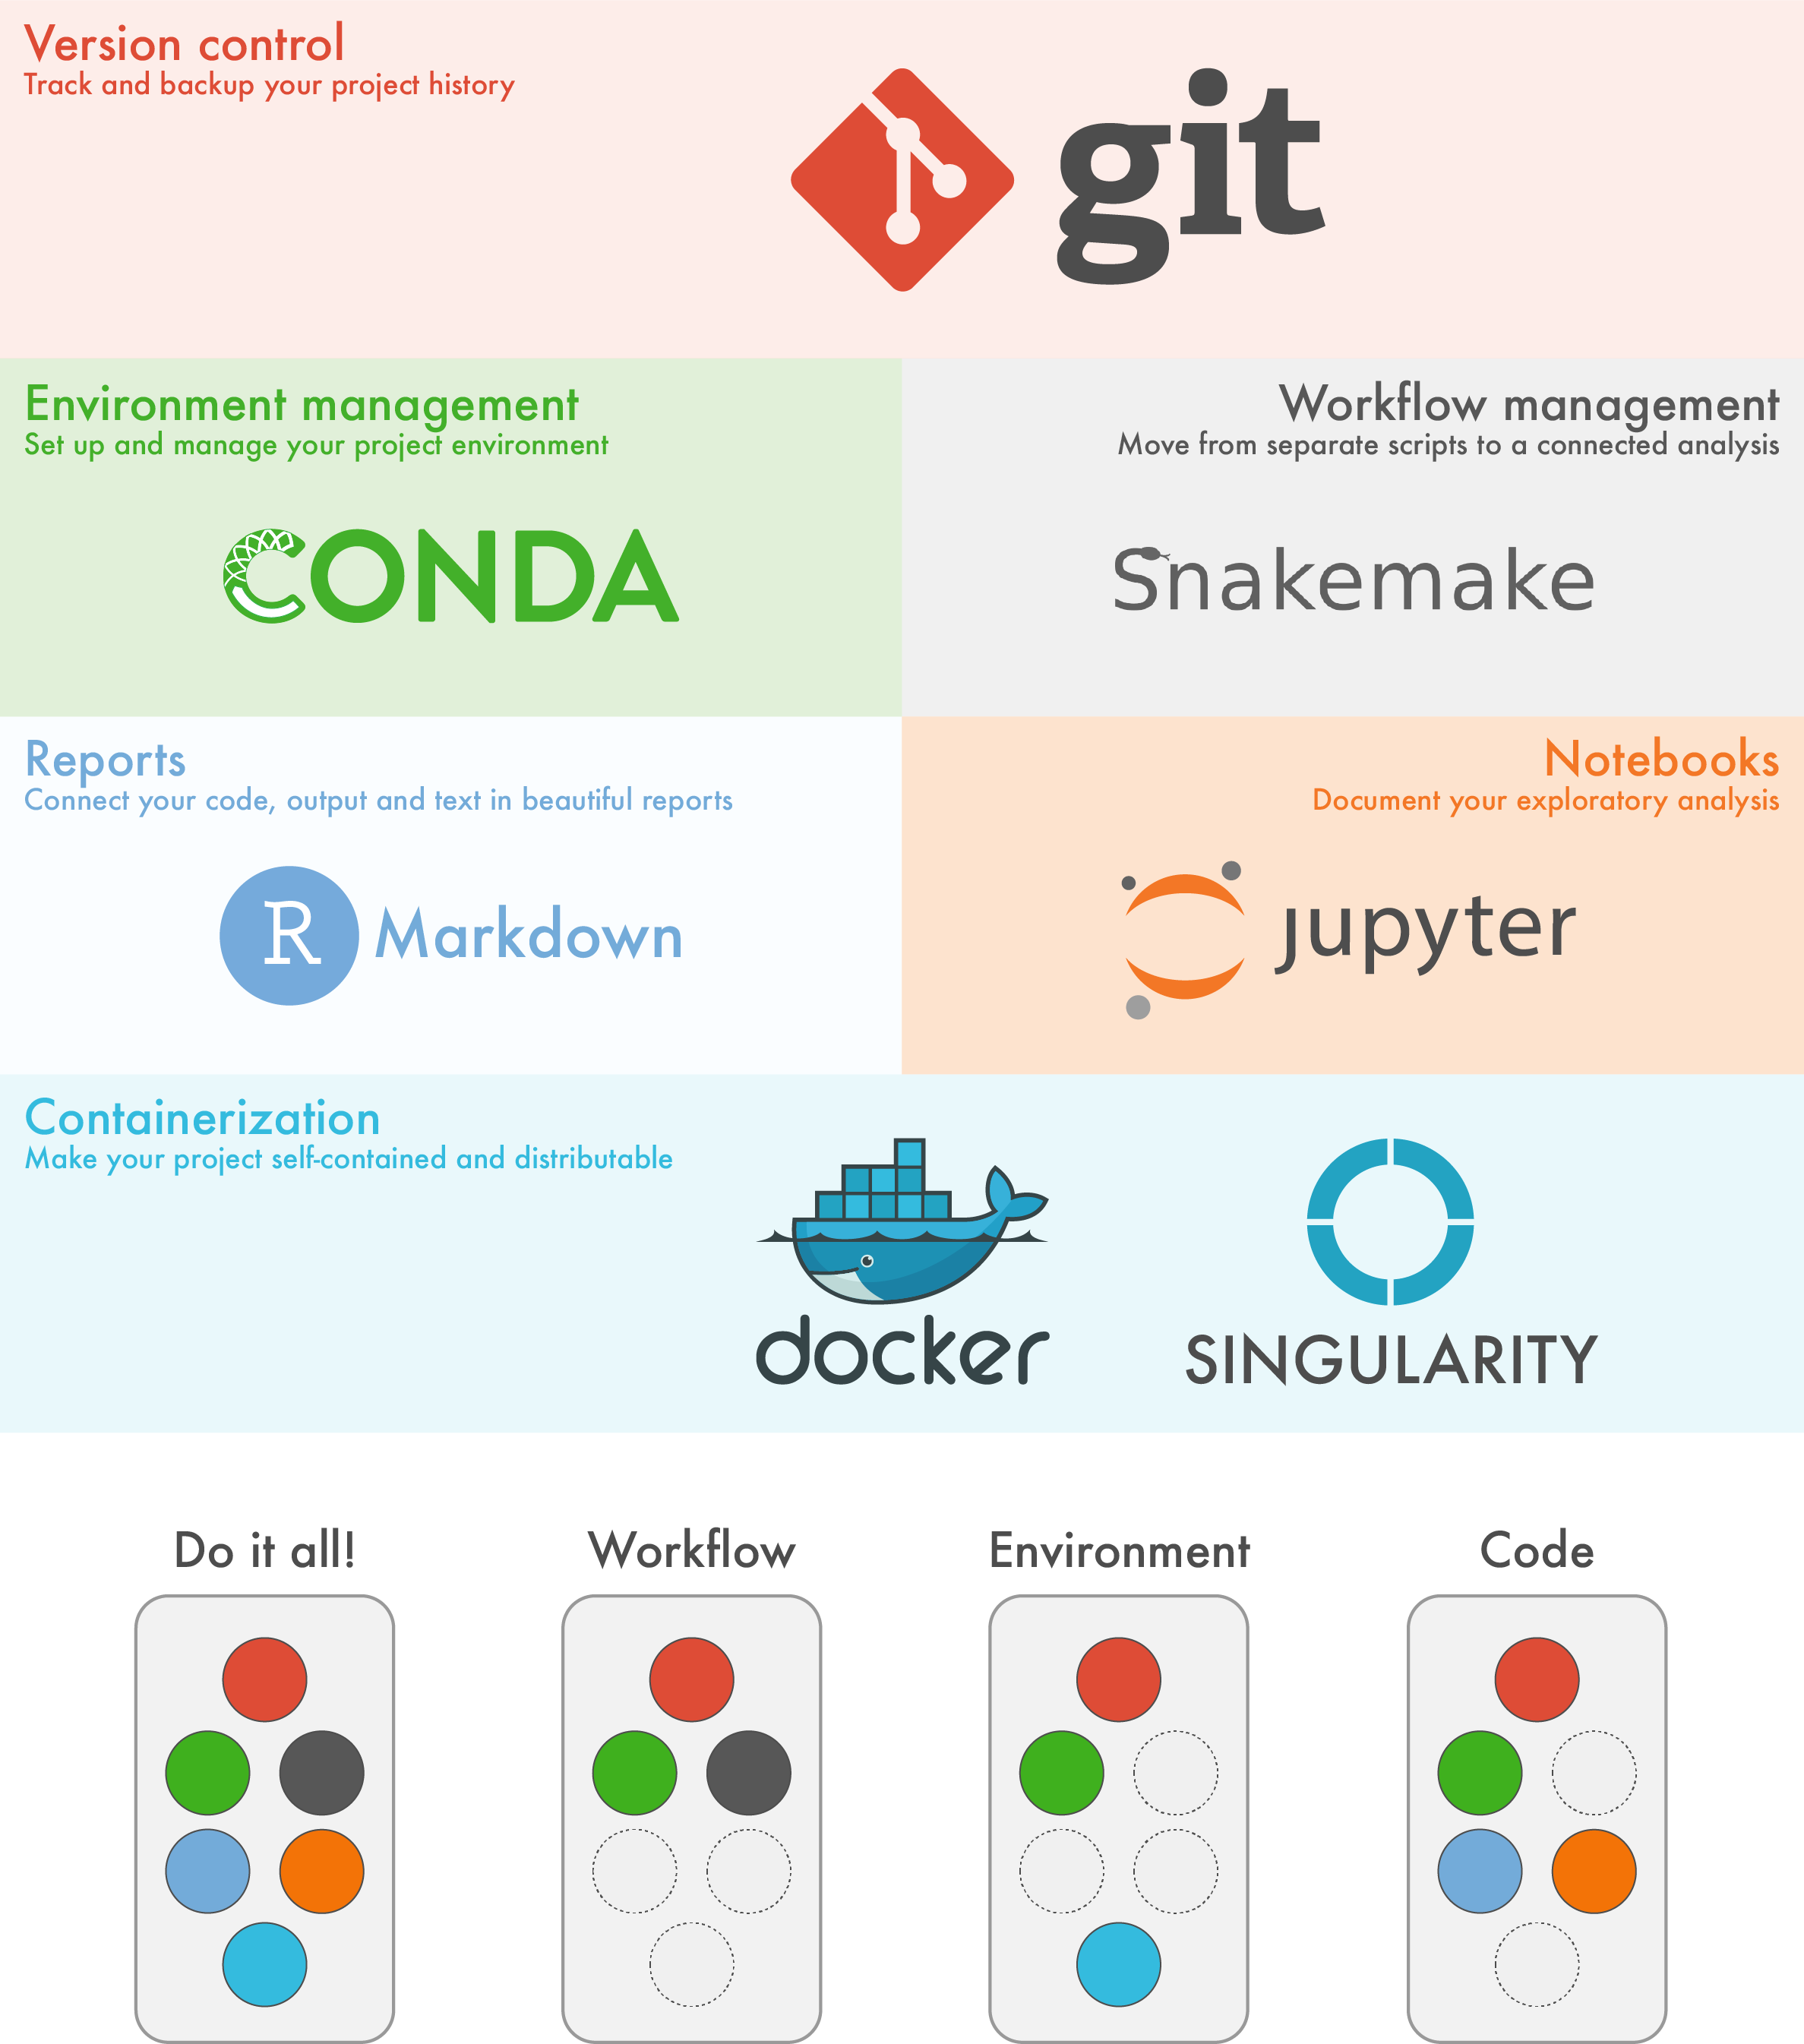
\includegraphics[scale=0.3]{images/tutorials_overview.png}
\end{textblock*}
\end{frame}

\begin{frame}{FAIR session with AuBi}
\begin{block}{Objectives}<1->
\begin{itemize}
\item Discover FAIR practices
\item Discover tools for best practices
\item Use tool and best practices in practice sessions
\item<2-> 5 sessions for courses and practices
	\begin{itemize}[<2->]
	\item Day 1: Introduction to FAIR training and Git
	\item Day 2: Git practice
	\item Day 3: Encapsulation course
	\item Day 4: Encapsulation training
	\item Day 5: Documentation course and training
	\end{itemize}
\end{itemize}
\end{block}
\end{frame}

\section{Training content}
\begin{frame}
\begin{block}{Contents}
\begin{itemize}
\item<1-> Introduction to FAIR practices
\item<2-> Code control using Git \faGit* 
	\begin{itemize}[<2->]
	\item Git environment
	\item Gitlab and Github \faGithub \faGitlab
	\end{itemize}
\item<3-> Encapsulation process
	\begin{itemize}[<3->]
	\item Conda environment and packages use 
\includegraphics[scale=0.07]{images/conda_logo.pdf}
	\item Containers as docker \& singularity \faDocker 
	\item Reproducible workflow using snakemake 	
\includegraphics[scale=0.05]{images/snakemake_logo.png}
	\end{itemize}
\item<4-> Literate programming and documentation
	\begin{itemize}[<4->]
	\item Markdown syntax \faMarkdown
	\item Rmarkdown for R \faRProject 
	\item Jupyterlab for Python \faPython
	\end{itemize}
\end{itemize}
\end{block}
\end{frame}


\end{document}


